\documentclass[11pt,a4paper]{article}
\voffset = -80pt
\textheight = 680pt


\usepackage{graphicx,array,amsmath,braket,amsfonts,rotating}

\begin{document}

\title{The Reconfigurable Waveguide Array}
\date{\today}
\author{Robert Chapman\\Quantum Photonics Laboratory, CUDOS, University of Sydney}
\maketitle

\subsection*{Introduction}

Quantum walks have been highlighted as a method of exploring quantum interference (\cite{Aharonov},\cite{Peruzzo}) and performing quantum simulations (\cite{Schreiber}). A quantum walk can be performed in a photonic lattice, utilizing the evanescent coupling between narrowly separated waveguide and spontaneous parametric down conversion as a source of indistinguishable photon pairs. 

\subsection*{Quantum Walk Hamiltonian}

The Hamiltonian to describe a quantum walk through an array of waveguides is based on the coupling coefficient between each waveguide and the propagation coefficient, denoted $\beta$. The coupling coefficients are given as $C_{ij}$, where $C^{-1}$ is the distance to couple from waveguide $i$ to waveguide $j$ and, in the reconfigurable array, will be a function of the voltage $V$ applied to the electrodes between. Considering only nearest neighbour coupling and an array of $N$ waveguides, the Hamiltonian is given as

\begin{equation}
\mathcal{H} _{array} = \begin{pmatrix}
\beta_0 & C_{0,1} & 0 & 0 & \dots& 0 & 0 \\
C_{1,0} & \beta_1 & C_{1,2} & 0 & \dots & 0 & 0 \\
0 & C_{2,1} & \beta_2 & C_{2,3} & \dots & 0 & 0 \\
0 & 0 & C_{3,2} & \beta_3 & \dots & 0  & 0 \\
\vdots & \vdots & \vdots & \vdots &  & \vdots & \vdots \\
0 & 0 & 0 & 0  & \dots & \beta_{N-2} &  C_{N-2,N-1} \\
0 & 0 & 0 & 0  & \dots & C_{N-1,N-2} & \beta_{N-1}
\end{pmatrix}.
\label{Equation:H_array}
\end{equation}

\noindent Each coupling constant $C$ will be tunable by applying a voltage and the coupling between waveguides will be equal in both directions, ie. $C_{ij} = C_{ji}$. Applying voltages to alter the coupling coefficients will also have an affect on the propagations coefficients $\beta_i$.

The unitary of the waveguide array can be determined from evolving this Hamiltonian

\begin{equation}
\hat{U}_{array} = \exp(i\mathcal{H}_{array}z).
\end{equation}

A simulation of the propagation of light through a waveguide array is shown in figure (\ref{Figure:RSoft_Sim}) where the input is into the central waveguide.
 \\
\begin{figure}[h]
\makebox[\textwidth][c]{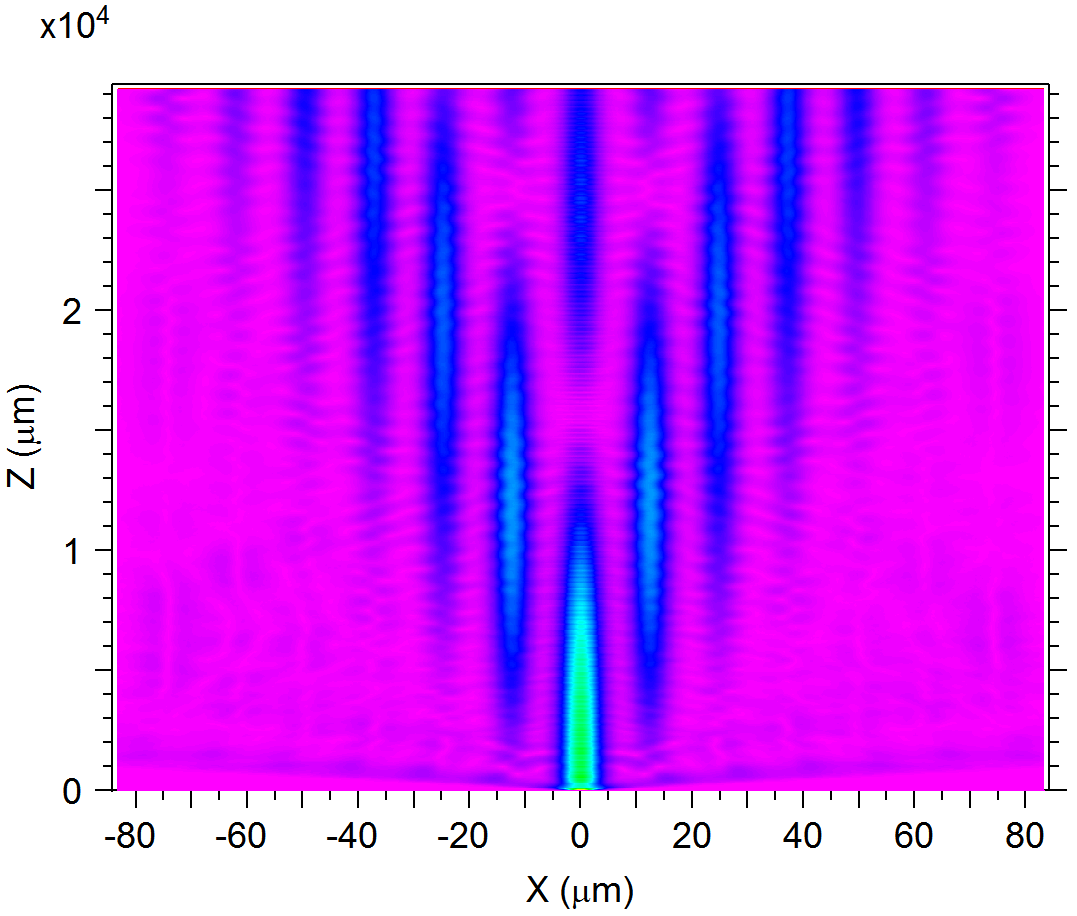
\includegraphics[width=0.8\textwidth]{RSoft_Sim}}
\caption{\small \textbf{Simulation.} Beam propagation method simulation of a 13 waveguide array with 12.4$\mu m$ spacing.}
\label{Figure:RSoft_Sim}
\end{figure}

\subsection*{Experiment Ideas}

Here is a list of projects that we could work together on performing on the reconfigurable waveguide array platform:

\begin{itemize}
\item Boson sampling / Hamiltonian mixing / Performing identity
\item Search/optimization algorithms
\item A general study of possible Hamiltonians
\end{itemize}

\noindent Here is a list of other ideas we will look into with this device:

\begin{itemize}
\item Perfect State Transfer
\item Controlled beam steering
\item Anderson localization with tunable noise
\item Optimizations for quantum simulations and quantum chemistry
\end{itemize}

\subsection*{Experimental Setup}

Photon pairs are produced via spontaneous parametric down conversion (SPDC) of a 404$nm$ laser to produce indistinguishable pairs of 808$nm$ photons. Coupling into fibre gives control and capability to couple through a v-groove fibre array with 127$\mu m$ pitch into the device. This source is stable and produces $\mathcal{O}(10^5)$ photon pairs per second.

To inject and retrieve photons from the waveguide array using commercially available v-groove fibre arrays requires the devices to have a fan-in and fan-out. These components will contribute to the coupling between the waveguides with a Hamiltonian of the form in equation (\ref{Equation:H_array}), however, has been engineered to have the same coupling coefficient between all waveguides. The complete unitary for the device will therefore be

\begin{equation}
\hat{U}_{total} = \hat{U}_{fan}\hat{U}_{array}\hat{U}_{fan},
\end{equation}

\noindent the device mask is shown in figure (\ref{Figure:Mask}).

Silicon single photon avalanche diode detectors are used in conjunction with an field programmable gate array in order to distinguish coincidence counts from single photon detection. 
 \\
\begin{figure}[h]
\makebox[\textwidth][c]{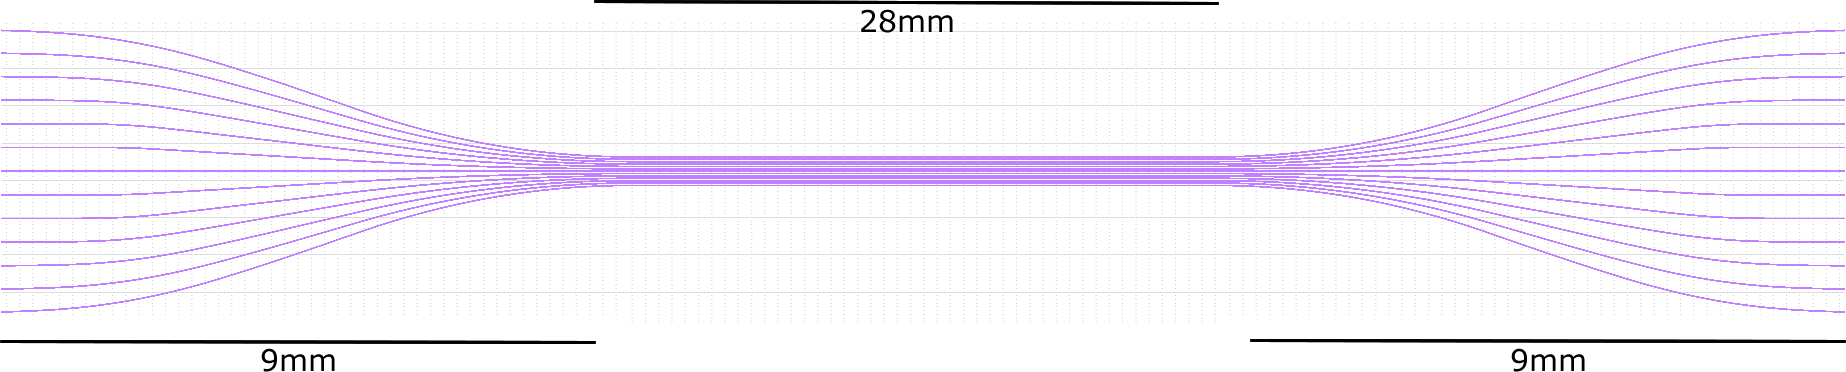
\includegraphics[width=0.8\textwidth]{Mask}}
\caption{\small \textbf{Device Mask.} Mask for waveguide array inc. fan-in and fan-out. Electrodes run along either side of each waveguide as shown in figure (\ref{Figure:RWA Electrode Design}).}
\label{Figure:Mask}
\end{figure}


%
%\begin{equation}
%\mathcal{H} _{fan} = \begin{pmatrix}
%\beta & C_{fan} & 0 & 0 & \dots& 0 & 0 \\
%C_{fan} & \beta & C_{fan} & 0 & \dots & 0 & 0 \\
%0 & C_{fan} & \beta & C_{fan} & \dots & 0 & 0 \\
%0 & 0 & C_{fan} & \beta & \dots & 0  & 0 \\
%\vdots & \vdots & \vdots & \vdots &  & \vdots & \vdots \\
%0 & 0 & 0 & 0  & \dots & \beta &  C_{fan} \\
%0 & 0 & 0 & 0  & \dots & C_{fan} & \beta
%\end{pmatrix}.
%\end{equation}
%
%\noindent The evolution of both these Hamiltonians needs to be performed in order to determine the unitary for the reconfigurable waveguide array.
%
%\begin{equation}
%\hat{U} = \exp(i\hat{H}z),
%\end{equation}
%
%\begin{equation}
%\hat{U}_{RWA} =  e^{(i\mathcal{H}_{fan}z_{f})}e^{(i\mathcal{H}_{RWA}z_{RWA})}e^{(i\mathcal{H}_{fan}z_{f})},
%\end{equation}
%
%\noindent where $z$ is the propagation distance of the Hamiltonian, $z_{f}$ is the propagation length of the fan-in/out and $z_{RWA}$ is the propagation length of the tunable array. This unitary can be applied to an input quantum state in order to determine the probability amplitudes at the outcome.
%
%The coupling coefficient $C_{i,j}(V)$ is found using the refractive indices of the waveguide and cladding, the separation of the waveguides and the wavelength of the light. The voltage applied simply alters the refractive indices.
%
%To describe two photons passing through the waveguide array, the unitary
%
%\begin{equation}
%\hat{U}_{RWA_2} = \hat{U}_{RWA}\otimes\hat{U}_{RWA},
%\end{equation}
%
%needs to be considered and the input state as
%
%\begin{equation}
%\psi_{in} = \psi_{1}\otimes\psi_{2}.
%\end{equation}
%



\subsection*{Device Details}

The reconfigurable waveguide array (RWA) consists of 13 titanium diffused 4$\mu m$ wide lithium niobate waveguides, with spacings ranging from 12.4$\mu m$ to 13.2$\mu m$ and a coupling length of 28000$\mu m$. Each waveguide has an electrode on either side. When a voltage is applied to a pair of electrode, the refractive indices of the waveguides and cladding change in opposing directions, as shown in figure (\ref{Figure:RWA Electrode Design}). Each electrode can be controlled individually with a maximum potential of around 6-7V and the refractive index will change according to

\begin{equation}
\Delta n = n^3r_{33}E,
\end{equation}

\noindent where $n$ is the refractive index of the waveguide, $r_{33}$ is the electro-optical coefficient of lithium niobate and $E$ is the electric field. This will give control over the coupling between adjacent waveguides and therefore a tunable Hamiltonian applied by the device.

\begin{figure}[h]
\makebox[\textwidth][c]{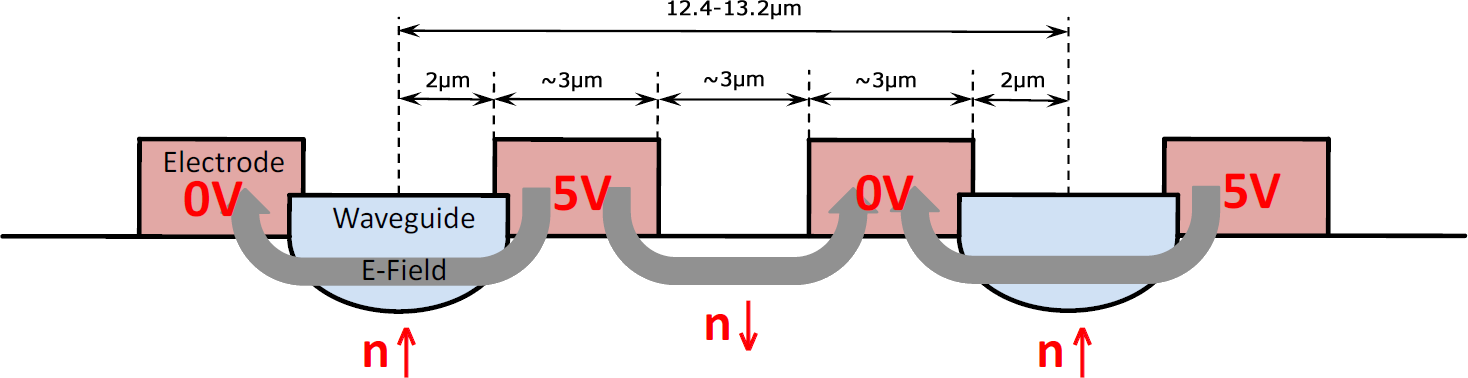
\includegraphics[width=1.2\textwidth]{Electrode_Design}}
\caption{\small \textbf{RWA Electrode Design.} Arrangement of the electrodes for the 13 waveguides in the RWA. Each electrode is controlled via a PCB which is, in turn, controlled via a PC.}
\label{Figure:RWA Electrode Design}
\end{figure}


\begin{thebibliography}{99}

\bibitem{Aharonov}\textit{Quantum random walks}; Y. Aharonov, L. Davidovich \& N. Zagury; Phys. Rev. A, Vol. 48 \textbf{2} (1993)

\bibitem{Peruzzo} \textit{Quantum Walks of Correlated Photons}; A. Peruzzo \textit{et al.}; Science, Vol. 329, pp.1500-1503 (2010)

\bibitem{Schreiber} \textit{A 2D Quantum Walk Simulation of Two-Particle Dynamics}; A. Schreiber \textit{et al.}; Science, Vol. 336, pp.55-58 (2012)

\end{thebibliography}

\end{document}